% Chapter Template

\chapter{Dataset Creation} % Main chapter title

\label{Chapter2} % Change 2 to a consecutive number; for referencing this chapter elsewhere, use \ref{Chapter2}

%----------------------------------------------------------------------------------------
%	SECTION 1
%----------------------------------------------------------------------------------------

\section{createDataset.py}

We created a text file, containing more than 1M data points in the form of (x, y), where x and y are real numbers. The generation of was biased toward the creation of three clusters. In other words, we chose randomly three centers (10, 25), (2, -9) and (-15, -35) and then, we generated the rest of the points around these, using some random distance following a skewed distribution.\\ \\
For this purpose we first found distances by using scipy.stats.skewnorm library and then we used these distance to choose random points as shown bellow.

\HRule \\[0.2cm] % Horizontal line
\begin{lstlisting}[language=Python]
from scipy.stats import skewnorm
import numpy as np
import matplotlib.pyplot as plt
import pandas as pd
from random import random, uniform
from math import sqrt, pow


# get random points that follows skew distribution and 
# use them as distance
def skew():

	fig, ax = plt.subplots(1, 1) # This function creates 					 # a figure and a grid of subplots

	a = 5 # skewness parameter, when a = 0 the 		 
	      # distribution is identical to a normal distribution
	
	d = skewnorm.rvs(a, size=350000)
	
	 # histogram of numbers generated
	plt.show()
	ax.hist(d, density=True, histtype='stepfilled', alpha=0.2)

	# return all the numbers generated with skew distribution
	return d 


# get random point from a circle that has as center 
# given centroid and as radius the distance found in 
# skew() function
def get_random_point(x, y, cluster):

	array = []
	distance = skew()
	
	for d in distance:
		while True:
		angle = random() * math.pi * 2
		x1 = x + math.cos (angle ) * d
		y1 = y + math.sin (angle ) * d
		
		if [x1, y1, cluster] not in array:
			print('yeah')
			break # if the pair of (x1,y1) exist find another pair of (x1,y1)
		
		array.append([x1, y1, cluster])
		print(x1, y1, cluster, len(array))
		
	return array


if __name__ == "__main__":
	
	# pre-define three centers for clusters
	centers = [[10, 25], [2, -9], [-15, -35]]
	data = [] # array with all the final data
	
	for center in centers:
		# concat the results of these
		# three clusters in one array
		data = data + get_random_point ( center[0], center[1], centers.index(center)) print(len(data))
		print(data)
	
	plt.scatter([item[0] for item in data], [item[1] for item in data], c=[item[2] for item in data])
	plt.show()
	
	df = pd.DataFrame(data)
	df.drop(df.columns[[2]], axis=1, inplace=True)
	df.to_csv("datasetNew", header=False, index= False, sep="," )

\end{lstlisting}
%----------------------------------------------------------------------------------------
%	SECTION 2
%----------------------------------------------------------------------------------------
\newpage
\section{Plot of data points}
The distances were generated with the use of skew() function and follow skew distribution as left image reveals. \\
The data points that were generated are shown in the right image.

\HRule \\[0.2cm] % Horizontal line
	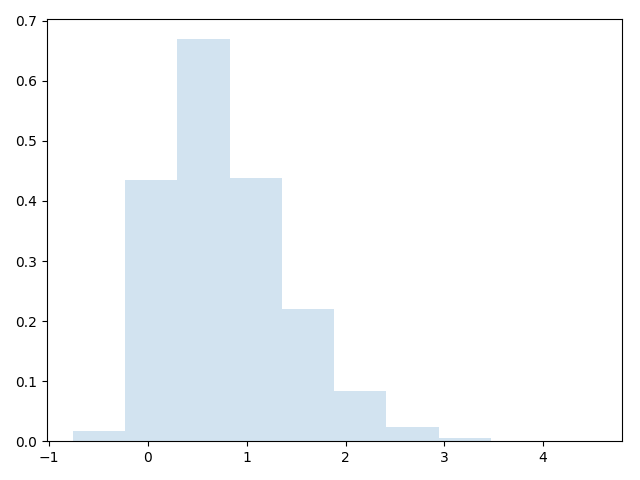
\includegraphics[width=0.5\textwidth]{../images/histogramOfDistancePoints.png}
	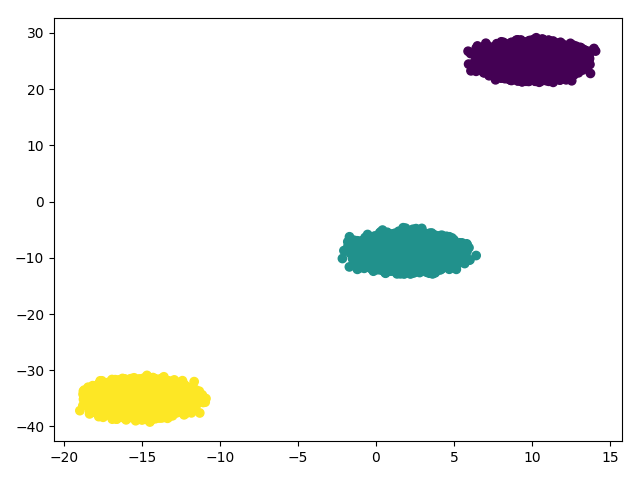
\includegraphics[width=0.5\textwidth]{../images/clustersCreatedImage.png}\\

